\documentclass[11pt]{article}

\usepackage{maiacustom}

\begin{document}

\psettitle{Banco de questões de astronomia}

Estas questões foram produzidas/selecionadas cuidadosamente com o objetivo de preparar os estudantes para o processo seletivo de astronomia no Brasil. Algumas questões não são de autoria própria e estão devidamente sinalizadas por () antes do enunciado. O template do banco de questões é o mesmo do Professor \text{Kevin Zhou}. Seu trabalho é valioso, e diversas ideias desta lista podem ser encontradas em seus Handouts.

% \begin{psidea}{Título da Ideia}{}
% Ideia
% \end{psidea}

% \begin{psexample}{Título do Exemplo}{}
% Exemplo
% \end{psexample}

% \begin{pssolution*}{}{}
% Solução
% \end{pssolution*}

% \begin{psremark*}{Título da Observação}{}
% Observação
% \end{psremark*} 
\section{Óptica e Telescópios}

\pts{3}
    \begin{pproblem} Um telescópio Kepleriano possuí duas lentes convergentes. A primeira possuí o raio de curavtura das duas faces igual a \(R = 2\text{ m}\) e a segunda possuí ambos os raios de curvatura igual a \(r = 0,5 \text{ m}\). Considerando que ambas as lentes possuem espessura desprezivel e são feitas de um material com indíce de refração \(n=1,4\). Calcule o diâmetro e o aumento do telescópio sabendo que este telescópio é um f/12.
    \begin{pssolution*}{}{}
        O Foco do telescópio será a soma dos focos individuais de cada lente. Utilizando a equação dos fabricantes de lentes, 
        \[\frac{1}{f} = \left(\frac{n_{\text{lente}}}{n_{\text{meio}}}-1\right)\left(\frac{1}{R_1}+\frac{1}{R_2}\right)\]

        Sejam \(a\) e \(b\) as lentes da objetiva e da ocular, reespectivamente, obtemos, 
        
        \[f_a = 2,50 \text{ m}\ ; \ f_b = 0,625\text{ m}\]

        Portanto, o foco do telescópio será, \[f = f_a+f_b = 3,125\text{ m}\]. Usando que o mesmo é \(f/12\), obtemos
        \[\boxed{D = f/12 = 260 \text{ mm}}\]
    \end{pssolution*}
    \end{pproblem}


\pts{5}
    \begin{pproblem}
        Nessa questão, vamos nos familiarizar com uma das ferramentas mais poderosas da óptica, a \textit{óptica geométrica}. O objetivo dessa ferramenta é modelar lentes e espelho em forma de matrizes. Isso é muito útil para resolver questões envolvendo associações de diversas lentes e é um método de resolver problemas de óptica geométrica (praticamente) sem usar geometrica. Mas para isso, se atente as seguintes definições na imagem a seguir

        \begin{figure}[H]
            \centering
            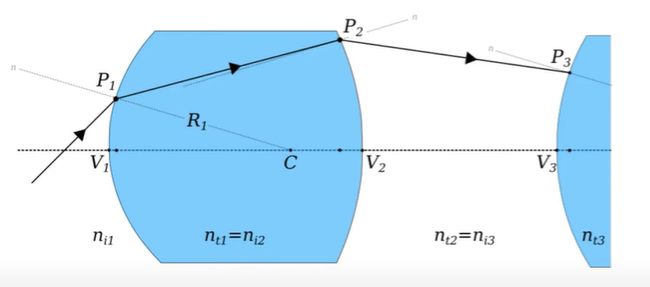
\includegraphics[width=0.9\linewidth]{imagens/lentes1.png}
            \caption{Esquema 1}
        \end{figure}

        Todas as linhas pontilhadas são paralelas ao eixo óptico, representado pela seta horizontal. É denotado por \(P_k\) o ponto onde a luz passa de um meio para o outro, \(y_k\) a coordenda vertical do ponto \(P_k\). São utilizados os subscritos \(i\) e \(t\) para se referir a incidente e transmitido, reespectivamente, então, por exemplo, \(\alpha_{i,k}\) é o ângulo que o raio de incidente luz faz com a horizontal no ponto \(P_k\), já o ângulo \(\alpha_k\) é o ângulo entre o ponto \(P_k\) e o centro da lente \(k\). Por exemplo, na figura, o ângulo \(\alpha_1\) é repsetenado por \(V_1\hat{C}P_1\).
        

        Para essa questão, vamos considerar que todos os ângulos de interesse são pequenos, de modo que \(\tan\theta \approx \sin\theta \approx \theta\).
        \begin{alternativas}
            \item Partindo da Lei de Snell, encontre uma relação entre \(n_{i,1}\), \(n_{t,1}\), \(\alpha_1\), \(\alpha_{i,1}\) e \(\alpha_{t,1}\).
        
            \item Encontre uma relação para \((1) \ n_{t,1}\alpha_{t,1}\) e \((2) \ y_{t,1}\). Deixe suas respostas em função de \(n_{i,1}\), \(\alpha_{i,1}\), \(y_{i,1}\) e \(\mathcal{D}_1\), para
            \[\mathcal{D}_1 = \frac{n_{t,1}-n_{i,1}}{R_1}\]

        Agora vamos para mais uma definição, seja o vetor \(\mathbf{r}_{t,1}= (n_{t,1}\alpha_{t,1}, \ y_{t,1})\) e \(\mathbf{r}_{i,1}= (n_{i,1}\alpha_{i,1}, \ y_{i,1})\).
        
            \item É possível escrever as duas equações que encontramos no item anterior na forma matricial, de forma:
            \[\mathbf{r}_{t,1}=\mathcal{R}_1\mathbf{r}_{i,1}\]
            Encontre a matriz \(2\times 2\) equivalente à \(\mathcal{R}_1\).

        Nosso interesse agora é encontrar as relações entre os pontos \(P_2\) e \(P_1\).

            \item Encontre uma equação para \(n_1\alpha_{i,2}\) e \(y_{i,2}\). Utilizando o raciocínio do item anterior, deixe sua resposta na forma
            \[\mathbf{r}_{i,2}=\Gamma_{2,1}\mathbf{r}_{t,1}\]
            Onde \(\Gamma_{2,1}\) também é uma matriz \(2\times 2\). Deixe sua resposta em função da espessura da lente, \(d_{2,1}\).

            \item Definimos a matriz da lente, \(\mathcal{A}_{2,1}\) da seguinte equação:
            \[\mathbf{r}_{t,2} = \mathcal{A}_{2,1}\mathbf{r}_{i,1}\]
            De modo que

            \[\mathcal{A}_{2,1} = \begin{pmatrix}
                a_{11} & a_{12} \\
                a_{21} & a_{22} \\
            \end{pmatrix}\]

            Encontre explicitamente \(\mathcal{A}_{2,1}\). Isso é de extrema importancia, pois descreve o raio de luz que sai da lente em função do raio que entra.

            \item Dentre todas as propriedades da matriz da lente, a mais curiosa delas é que o termo \(a_{12}\) é proporcional a \(-1/f\) onde \(f\) é o foco da lente. Prove esse resultado. (Dica: você consiguira escrever \(-a_{12}\) com uma equação bem conhecida da óptica).
        
        Agora, vamos colocar a mão na massa e fazer utilizações praticas da óptica matricial.

            \item Refaça o exercício anterior utilizando óptica matricial.
        
            \item Considere o seguinte esquema:
                \begin{figure}[H]
                    \centering
                    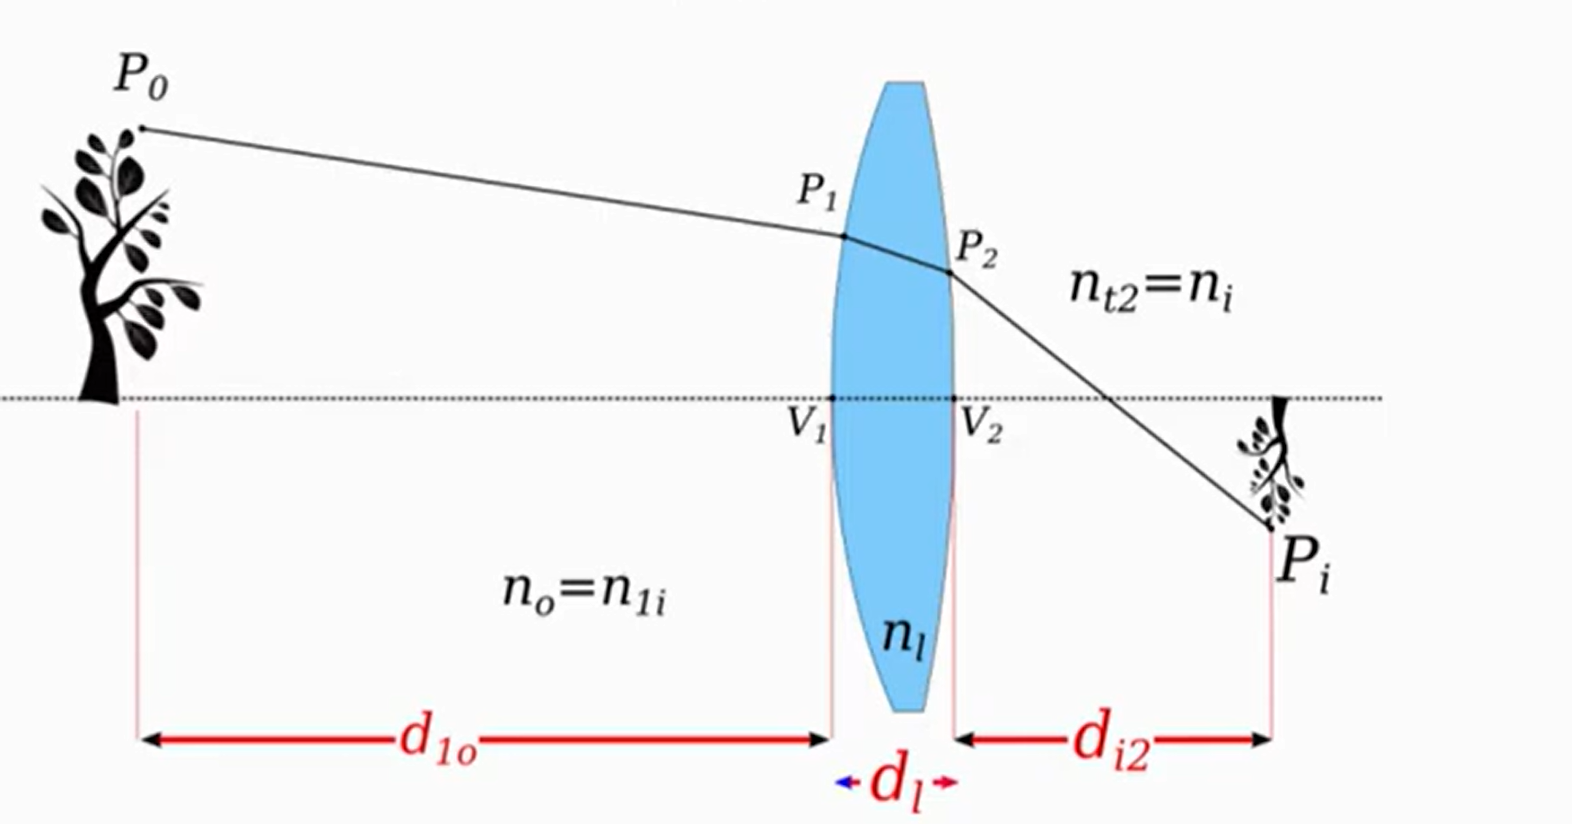
\includegraphics[width=0.9\linewidth]{imagens/lentes2.png}
                    \caption{Esquema 2}
                \end{figure}
                 Ecnontre \(y_i\) em função de \(y_0\) e dos dados na imagem.
                 
            \item Se a lente estiver entre dois meios diferentes, \(n_{i,1} \ne n_{t,2}\) temos a seguinte relação:
            \[a_{12} = -\frac{n_{i,1}}{f_0}=-\frac{n_{t,2}}{f_I}\]
                Utilizando-se disse, refaça a questão anterior, considerando que entre as duas lentes á água de \(n_w = 4/3\).
        
            \item Um arranjo muito comum de lentes é a Objetiva de Tessar, presente em muitas cameras pela sua eficiencia em diminuir efeitos de aberração e astigmatismo. O Arranjo tem a seguinte forma:
                \begin{figure}[H]
                    \centering
                    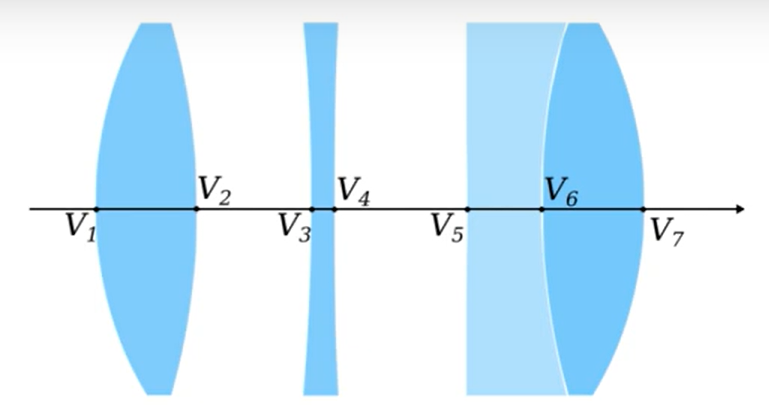
\includegraphics[width=0.7\linewidth]{imagens/lentes3.png}
                    \caption{Esquema Objetiva Tessar}
                \end{figure}
                Encontre a Matrix da Lente equivalente, \(\mathcal{A}_{1,7}\) em função de \(\mathcal{R}_i\) e \(\Gamma_{i,j}\).
        \end{alternativas}
    \begin{pssolution*}{}{}
        \begin{alternativas}
            \item A lei de Snell nos diz que \(n_{i,1}\theta_{i,1} = n_{t,1}\theta_{t,1}\). Onde \(\theta\) são os ângulso que a luz faz com a normal. Note que podemos escrever ambos os ângulos \(\theta\) como:
            \[\theta_{i,1} = \alpha_1 + \alpha_{i,1}, \ \ \theta _{t,1} = \alpha_1 + \alpha_{t,1}\]

            Logo, a relação que procuramos é 

            \[\boxed{n_{i,1}(\alpha_1+\alpha_{i,1}) = n_{t,1}(\alpha_1+\alpha_{t,1})}\]

            \item Substituindo \(\alpha_1 = y_1/R_1\), temos
            
            \[n_{i,1}(y_1/R_1+\alpha_{i,1})=n_{t,1}(y_1/R_1 +\alpha_{t,1})\]

            isolando \(n_{t,1}\alpha_{t,1}\)

            \[n_{t,1}\alpha_{t,1} = n_{i,1}\alpha_{i,1}+ \frac{y_1}{R_1}(n_{i,1}-n_{t,1})\]

            Em termos de \(\mathcal{D}_1\) 

            \[n_{t,1}\alpha_{t,1} = n_{i,1}\alpha_{i,1} - y_1\mathcal{D}_1\]

            Note que \(y\) não muda imediatamente após a transmissão da luz. Logo \(y_1\equiv y_{i,1}\equiv y_{t,1}\).

            \item Na forma matricial
            
            \[\left(\begin{matrix}
                n_{t,1}\alpha_{t,1} \\
                y_{t,1}\\
            \end{matrix}\right) = \left(\begin{matrix}
                1 & - \mathcal{D}_1 \\
                0 & 1
            \end{matrix}\right)\left(\begin{matrix}
                n_{i,1}\alpha_{i,1} \\
                y_{i,1}\\
            \end{matrix}\right)\]

            Assim, nossa matriz \(\mathcal{R}_1\), também conhecida como matriz refração é dada por:

            \[\boxed{\mathcal{R}_1 = \left(\begin{matrix}
            1 & -\mathcal{D}_1 \\
            0 & 1 \\
            \end{matrix}\right)}\]

        \item Primeiro, vamos achar a altura do ponto \(2\). Seja \(d_{21}\) a espessura da lente. Utilizando trigonometria obtemos
        
        \[y_{i,2} = y_{t,1} + \alpha_{t,1}d_{21}\]

        Temos que \(\alpha_{t,1}\) e \(\alpha_{i,2}\) são alternos internos. Ou seja \(\alpha_{t,1}=\alpha_{i,2}\). Como o indice de refração dentro da lente é constante (\(n_{i,2} = n_{t,1}\)), temos \(n_{t,1}\alpha_{t,1} = n_{i,2}\alpha_{i,2}\). Colocando as duas expressoões na forma matricial obtemos, 

        \[\begin{pmatrix}
            n_{i,2}\alpha_{i,2}\\
            y_{i,2}\\
        \end{pmatrix}
        =
        \begin{pmatrix}
            1 & 0 \\
            \frac{d_{2,1}}{n_{t,1}} & 1 \\
        \end{pmatrix}
        \begin{pmatrix}
            n_{t,1}\alpha_{t,1} \\
            y_{t,1}\\
        \end{pmatrix}
        \]

        Portanto, podemos concluir que, 

        \[\boxed{\Gamma_{2,1} = \begin{pmatrix}
        1 & 0 \\
        \frac{d_{2,1}}{n_{t,1}} & 1 \\
        \end{pmatrix}}\]

        \item Juntando as expressões encontradas anteriormente, 
        \[\mathbf{r}_{i,2} = \Gamma_{2,1} \mathbf{r}_{t,1}\]
        \[\mathbf{r}_{i,2} = \Gamma_{2,1} (\mathcal{R}_1\mathbf{r}_{i,1})\]

        E como vimos anteriormente, para irmos de \(\mathbf{r}_{i,k}\) para \(\mathbf{r}_{t,k}\) basta utilizarmos a matriz \(\mathcal{R}_k\), desse modo

        \[\mathbf{r}_{t,2} = \mathcal{R}_2\Gamma_{2,1}\mathcal{R}_1\mathbf{r}_{i,2}\]

        Logo, a matrix \(\mathcal{A}_{2,1}\) é a multiplicação da matriz \(\mathcal{R}_2\) pela matriz \(\Gamma_{2,1}\) pela matriz \(\mathcal{R}_1\). Explicitamente, 

        \[\mathcal{A}_{2,1} = \left(\begin{matrix}
            1 & -\mathcal{D}_2 \\
            0 & 1 \\
            \end{matrix}\right)\begin{pmatrix}
        1 & 0 \\
        \frac{d_{2,1}}{n_{t,1}} & 1 \\
        \end{pmatrix}
        \left(\begin{matrix}
            1 & -\mathcal{D}_1 \\
            0 & 1 \\
            \end{matrix}\right)\]
        \end{alternativas}

        Com muita determinação, podemos resulver essa conta, obtendo, 

        \[\boxed{
        \mathcal{A}_{2,1} = 
        \begin{pmatrix}
        1 - \frac{\mathcal{D}_2d_{2,1}}{n_{t,1}} & - \mathcal{D}_1 - \mathcal{D}_2 + \frac{\mathcal{D}_1\mathcal{D}_2d_{2,1}}{n_{t,1}} \\
        \frac{d_{2,1}}{n_{t,1}} & \frac{\mathcal{D}_1 d_{2,1}}{n_{t,1}}\\
        \end{pmatrix}
        }
        \]

        \item Trabalhando com o termo \(a_{1,2}\), temos, 
        
        \[a_{1,2} = -\mathcal{D}_1 - \mathcal{D}_2 + \frac{\mathcal{D}_1\mathcal{D}_2d_{2,1}}{n_{t,1}}\]

        Substituindo \(\mathcal{D}_k\), temos, 

        \[a_{1,2} = -\frac{n_{t,1}-n_{i,1}}{R_1} - \frac{n_{t,2}-n_{i,2}}{R_2} + \frac{(n_{t,1}-n_{i,1})(n_{t,2}-n_{i,2})d_{2,1}}{n_{t,1}R_1R_2}\]

        Note que, para a nossa situação, \(n_{i,1}\) e \(n_{t,2}\) correspondem aos indices de refração do meio, já \(n_{t,1}\) e \(n_{i,2}\) correspondem aos indices de refração da lente, que serão denotados por \(n_m\) e \(n_l\) reespectivamente. Dessa maneira, 

        \[a_{1,2} = -\frac{n_{l}-n_{m}}{R_1} - \frac{n_{m}-n_{l}}{R_2} + \frac{(n_{l}-n_{m})(n_{m}-n_{l})d_{2,1}}{n_lR_1R_2}\]

        \[a_{1,2} = - (n_l-n_m)\left(\frac{1}{R_1}-\frac{1}{R_2}\right) - \frac{(n_l-n_m)^2 d_{2,1}}{n_lR_1R_2}\]

        \[a_{1,2} = -(n_l-n_m)\left(\frac{1}{R_1}-\frac{1}{R_2} + \frac{(n_l-n_m)d_{2,1}}{n_l R_1R_2}\right)\]

        Isso tem formato identico a equação dos fabricantes de lentes (para espessuras não desprezíveis). 

        \[\frac{1}{f} = \left(\frac{n_l}{n_m}-1\right)\left(\frac{1}{R_1}-\frac{1}{R_2} + \frac{(n_l-n_m)d_{2,1}}{n_l R_1R_2}\right)\]

        Assim, podemos concluir que

        \[\boxed{a_{1,2} = -\frac{n_m}{f}}\]

\end{pssolution*}

\end{pproblem}

\pts{2}
\begin{pproblem}
    A teoria ondulatória da luz demonstra que um foco perfeito não é possível devido aos efeitos de difração associados à abertura finita da lente. Essa falta de foco perfeito impede que objetos muito próximos sejam distinguidos. Este problema pode ser estudado de dois pontos de vista diferentes:

    A teoria ondulatória da luz prevê que uma lente de diâmetro $D$ não pode focar um feixe paralelo de luz com comprimento de onda $\lambda$ em um ângulo menor que o limite de difração:
    \begin{equation}
        \theta_m \approx 1.22 \frac{\lambda}{D}
    \end{equation}

    Considere agora uma abordagem quântica, os fótons que são focados pela lente. Esses fótons são conhecidos por terem passado em algum lugar dentro de um raio do centro da lente. A incerteza na posição $x$ está associada a uma incerteza no componente $x$ do momento do fóton. Consequentemente, um fóton que, na ausência dessa incerteza, teria sido trazido para o eixo óptico do plano focal, pode agora ser desviado por um ângulo $\theta \ll 1$.

    Considere o comprimento de onda de de Broglie $\lambda = \frac{h}{p}$. Encontre um limite para $\theta$.

    \textbf{DICA:} o princípio de incerteza de Heisenberg, relaciona a impressição entre as medidas de momento e posição de uma particula por 
    \[\Delta p_x \Delta x = \frac{\hbar}{2}\]

\begin{pssolution*}{}{}
    O momento de um fóton é dado por \(p = h/\lambda\) e sabemos que o foton possui \(\Delta x = D\) utilizando o princípio da incerteza de Heisenberg

    \[\Delta p_x = \frac{\hbar}{2D}\]

    Utilizando que \(\theta \approx \frac{\Delta p_x}{p}\), obtemos
    \[\boxed{\theta \approx\frac{\lambda\hbar}{2D h} = \frac{1}{4\pi}\frac{\lambda}{D}}\]
\end{pssolution*}
\end{pproblem}

\pts{3}
\begin{pproblem} (Apostila Magna)
    Prove que a quantia \(n_iR_i\sin \theta_i\) para cascas esféricas adjacentes entre si, em que \(n_i\) é o índice de refração da i-ésima casca esférica, \(\theta_i\) é o ângulo que o raio de luz faz com a normal da i-ésima casca esférica e \(R_i\) é o raio da i-ésima casca esférica, é uma invariante
    
\end{pproblem}

\pts{4}
\begin{pproblem}
    O indídice de refração da atmosfera de um planeta é dado por, 

    \[n(h) = \frac{n_0}{1+\epsilon h}\]

    Onde \(n_0\) e \(epsilon\) são constantes.

    \begin{alternativas}
        \item Um raio de luz atinge a atmosfera paralelamente a superfície, há uma altura \(h'\ll R\), como será a trajetória?
        \item Sabendo a trajetória do raio de luz, calcule o Raio do planeta.
    
        \textbf{Dica:} Você pode achar útil a seguinte relação, 

        \[\int \frac{t}{\sqrt{a-bt^2}}dt = -\frac{1}{b}\sqrt{a-bt^2}+C\]
    \end{alternativas}
\begin{pssolution*}{}{}
    \begin{alternativas}
        \item Defidindo \(ds = \sqrt{dx^2+dh^2}\) como sendo o elemnto infinitesimal de arco, temos, 
        \[\sin\theta = \frac{dx}{ds}, \ \ \cos\theta = \frac{dh}{ds}\]

        Como o meio é contínuo, podemos escrever, 

        \[n(h)\sin\theta(h)=cte\]

        Assim, 

        \[n\frac{dx}{ds} = K\]

        Substituindo \(n\), 

        \[\frac{dx}{ds} = \frac{K(1+\epsilon h)}{n_0}\]

        Porém, pela definição de \(s\), temos, 

        \[\left(\frac{dx}{ds}\right)^2 + \left(\frac{dh}{ds}\right)^2 = 1\]

        Substituindo \(dx/ds\), 

        \[\frac{dh}{ds} = \sqrt{1- \left(\frac{K(1+\epsilon h)}{n_0}\right)^2}\]

        Usando uma regra da cadeia, 

        \[\frac{dh}{dx} = \frac{dh/ds}{dx/ds} = \frac{\sqrt{1- \left(\frac{K(1+\epsilon h)}{n_0}\right)^2}}{\frac{K(1+\epsilon h)}{n_0}}\]

        Simplficando a expressão, 

        \[\frac{dh}{dx} = \frac{\sqrt{n_0^2 - K^2(1+\epsilon h)^2}}{K(1+\epsilon h)}\]

        Para resolver essa E.D.O, vamos criar a variável \(u = 1+\epsilon h\), de modo que, 

        \[dh = \frac{du}{\epsilon}\]

        Assim, 

        \[\frac{du}{dx} = \epsilon\frac{\sqrt{n_0^2 - K^2u^2}}{Ku}\]

        Separando os termos e integrando, 

        \[\int \frac{u}{\sqrt{n_0^2 - K^2u^2}} du = \frac{\epsilon}{K}\int dx\]
    
        A integral do lado esquerdo, é a mesma fornecida pela questão, assim, 

        \[-\frac{1}{K^2}\sqrt{n_0^2-K^2u^2} = \frac{\epsilon}{K}x + C\]

        Trabalhando nessa expressão, 

        \[\sqrt{n_0^2-K^2u^2} = -\epsilon K x - K^2C\]

        \[n_0^2-K^2u^2 = (\epsilon K x + K^2C)^2\]

        Substituindo \(u\), 

        \[n_0^2-K^2(1+\epsilon h)^2 = \epsilon^2K^2x^2 + 2\epsilon K^3 C x + K^4C^2\]

        Rearranjando os termos, 

        \[\epsilon^2K^2x^2 + 2\epsilon K^3 C x + K^2(1+\epsilon h)^2 = n_0^2 - K^4C^2 \]

        \[\epsilon^2x^2 + 2\epsilon K C x + (1+\epsilon h)^2 = n_0^2/K^2 - K^2C^2 \]

        Dividindo por \(\epsilon^2\), 

        \[x^2 + \frac{2KC}{\epsilon}x + \frac{K^2C^2}{\epsilon^2} + \left(h+\frac{1}{\epsilon}\right)^2 = \left(\frac{n_0}{\epsilon K}\right)^2\]

        Juntando o produto notável, 

        \[\boxed{\left(x + \frac{KC}{\epsilon}\right)^2+\left(h+\frac{1}{\epsilon}\right)^2 = \left(\frac{n_0}{\epsilon K}\right)^2}\]
   
        Que é justamente a equação de um círculo de raio \(\frac{n_0}{\epsilon K}\) e centro \(C = (-\frac{KC}{\epsilon}, \ - \frac{1}{\epsilon})\).

        \item No caso de um raio que tangência o planeta, temos que o mesmo possuí \(\theta_0 = \pi/2\) e \(h_0=0\). Assim, utilizando, 
        
        \[n(h)\sin\theta(h) = n_0\sin\theta_0 = K\]

        Obtemos \(K = n_0\), assim, o raio do planeta é dado pelo raio da trajetória (O raio de luz é tangênte a superfície) e, portanto, 

        \[\boxed{R = \frac{1}{\epsilon}}\]
    \end{alternativas}
    
\end{pssolution*}
\end{pproblem}

\end{document}